\documentclass{jarticle}
\usepackage[dvipdfmx]{graphicx}
\usepackage{here}
\usepackage{listings}

\begin{document}

\title{課題1(再)}
\author{1029289895 尾崎翔太}
\date{2018/11/30}

\maketitle
\newpage

\section{アプリケーションの説明}
ビデオレンタルシステムである. 一般ユーザはあるビデオはどの店にあるか, ある店にはどんなビデオがあるかなどを検索できる. 店側は一般ユーザがどのビデオを借りているか, 及びその返却期限を確認できる.
\section{利用者の役割}
\begin{description}
\item[一般ユーザ] \leavevmode \\
このビデオレンタルショップを利用している消費者.
\item[店員] \leavevmode \\
このビデオレンタルショップが有している店の従業員.
\item[管理者] \leavevmode \\
このシステムの更新を行う人.
\end{description}
\section{役割ごとの機能}
\subsection{一般ユーザの機能}
\begin{description}
\item[ビデオ検索機能] \leavevmode \\
ビデオの名前や店の名前やジャンルで検索して, ヒットしたビデオのリストを得ることができる. また, その結果を発売年や長さでソートできる.
\item[店検索機能]
ある特定のビデオについて, それが置いてある店を得ることができる.
\item[利用状況確認機能] \leavevmode \\
自分がどのビデオを借りているか, 及びその返却期限を得ることができる.
\item[履歴確認機能] \leavevmode \\
自分の今までの利用履歴を確認できる.
\end{description}
\subsection{店員の機能}
\begin{description}
\item[利用状況確認機能] \leavevmode \\
自分が勤めている店について, どのビデオが誰に借りられていて, その返却期限はいつかを得ることができる.
\item[催促機能] \leavevmode \\
返却期限を過ぎている一般ユーザに返却を促すメールを送ることができる.
\end{description}
\subsection{管理者}
\begin{description}
\item[ビデオ管理機能] \leavevmode \\
新しいビデオを置いたり, 今まで置いてあったビデオを置かなくなったりしたときに追加/削除ができる.
\item[ユーザ管理機能] \leavevmode \\
新しいユーザを登録できる.
\item[店管理機能] \leavevmode \\
開店した店を追加したり, 閉店した店を削除したりできる.
\item[店員管理機能] \leavevmode \\
新しい店員を登録したり, 辞めた店員を削除したりできる.
\end{description}
\section{実体関連図}
\begin{figure}[htbp]
    \centering
    \caption{ER図}
    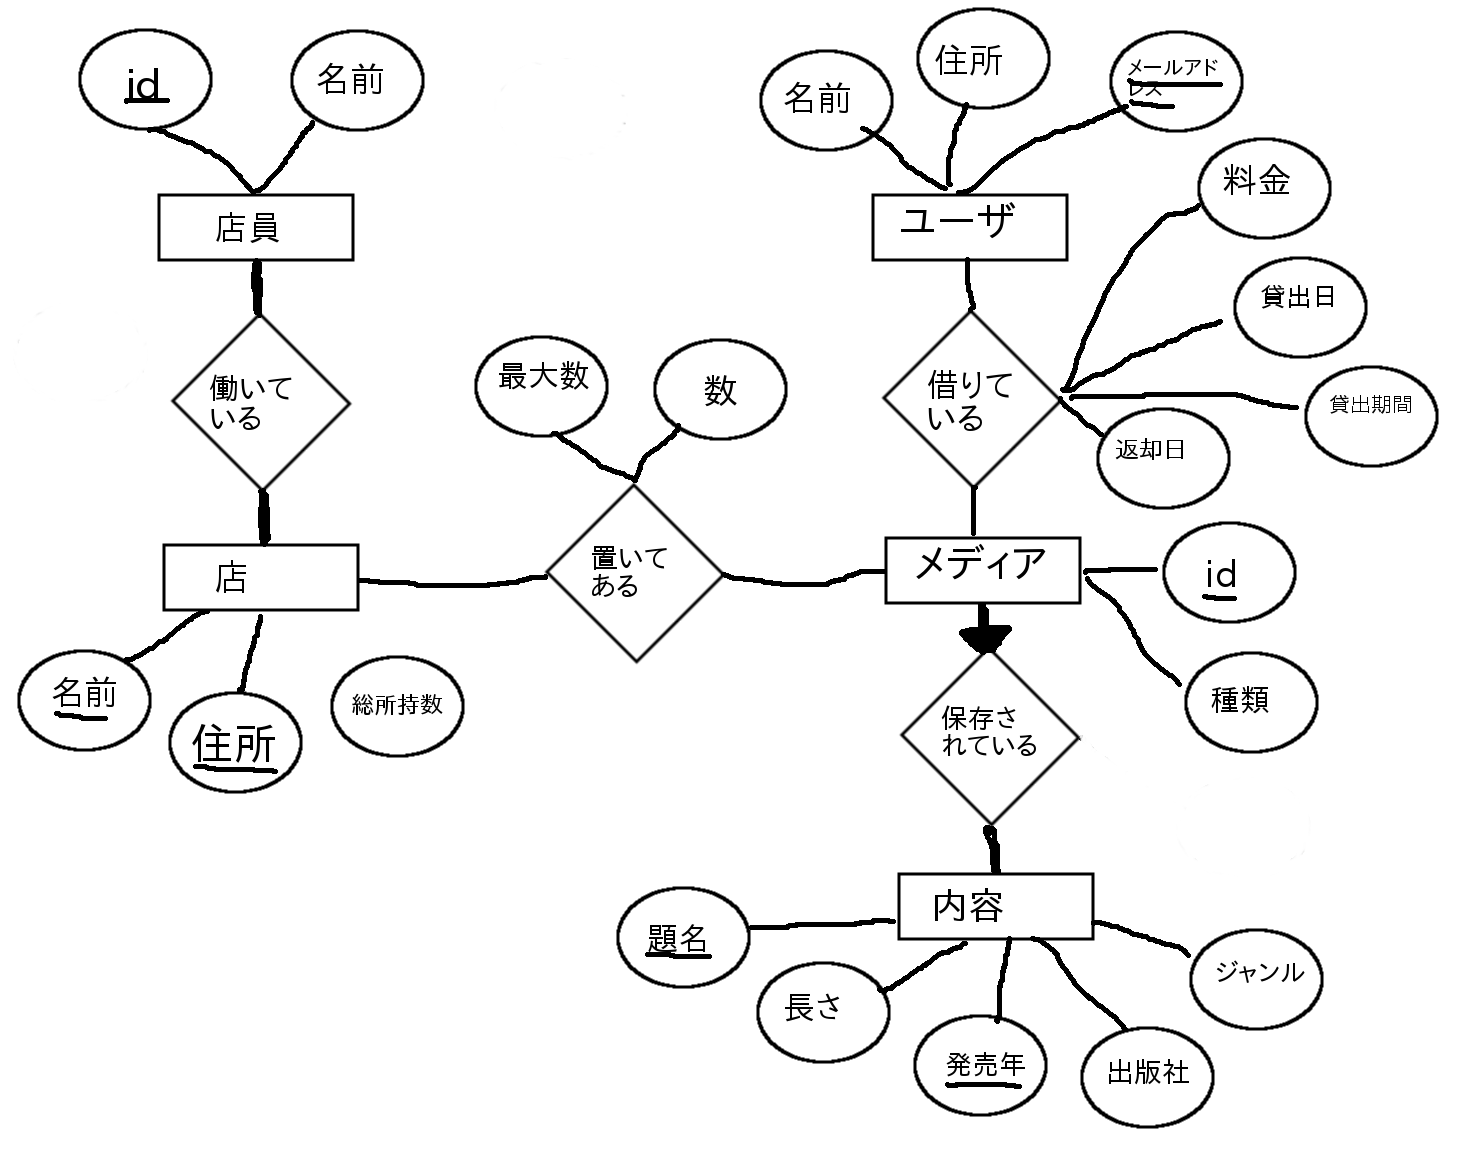
\includegraphics[width=15cm]{er.png}
\end{figure}
ER図は図1の通りである. 太線は参加制約, 矢印はキー制約を表している.
\subsection{実体}
図1の実体について説明する.
\begin{description}
\item[ユーザ] \leavevmode \\
一般ユーザに相当する実体である. 属性として名前と住所とメールアドレスを保持していて, キーはメールアドレスである. つまり, 登録の際にメールアドレスを必要とし, それで区別する.
\item[メディア] \leavevmode \\
このビデオレンタルシステムで取り扱うビデオが保存されているメディアに相当する実体である. 属性としてid, 種類を保持していて, キーはidである. 種類というのは, VHSやDVDやBlu-rayのことである.
\item[内容] \leavevmode \\
このビデオレンタルシステムで取り扱うビデオの中身に相当する実体である. 属性として題名, 長さ, 発売年, 出版社, ジャンルを保持していて, キーは題名と発売年である. 題名と発売年が同じで中身が違うビデオもひょっとするとあるかもしれないが, 今回はそんなものはないということにした.
\item[店] \leavevmode \\
このビデオレンタルシステムを使っているビデオレンタルショップの各店舗に相当する実体である. 属性として名前, 住所, 総所持数を保持していて, キーは名前と住所である. 総所持数とは, この店が所持しているメディアの合計である.
\item[店員] \leavevmode \\
店員に相当する実体である. 属性としてid, 名前を保持していて, キーはidである. このシステムにおいて名前の必要性は薄いのだが, 属性がキーだけだと寂しいので追加した.
\end{description}
\subsection{関連}
図1の関連について説明する.
\begin{description}
\item[借りている] \leavevmode \\
ユーザがビデオを借りていることを表す関連である. 属性として料金, 貸出日, 貸出期間, 返却日を保持している. ここにおける返却日は, ここまでに返さなければならない日のことである.
\item[置いてある] \leavevmode \\
ビデオが店に置いてあることを表す関連である. 属性として最大数, 数を保持している. 最大数はこの店にこのビデオが最大でいくつ置いてあるかを表していて, 数は今現在, 借りられているものを除いて, この店にこのビデオがいくつ置いてあるかを表している.  
\item[働いている] \leavevmode \\
店員が店で働いていることを表す関連である. 属性は保持していない. 参加制約があり, 店員は1つ以上の店で働いていなければならないし, 店も1人以上の店員が働いていなければならない.
\item[保存されている] \leavevmode \\
ビデオの内容がメディアに保存されていることを表す関連である. 参加制約があり, メディアには1つ以上の内容が保存されていなければならないし, 内容は1つ以上のメディアに保存されていなければならない. さらに, キー制約もあり, メディアは複数の内容を保存していてはならない.
\end{description}
\end{document}
